\begin{flushright} {\tiny {\color{gray} python\_codes/fieldstone\_131/text.tex}} \end{flushright}

%\lstinputlisting[language=bash,basicstyle=\small]{python_codes/fieldstone_131/keywords}

\begin{center}

\fbox{\textbf{\huge \color{teal} P}}
Codes at \url{https://github.com/cedrict/fieldstone/tree/master/python_codes/fieldstone_131}
\end{center}

\par\noindent\rule{\textwidth}{0.4pt}

{\sl This stone was developed in collaboration with M. Blasweiler and J. Wolbers}. 
\index{contributors}{M. Blasweiler}
\index{contributors}{J. Wolbers}

\par\noindent\rule{\textwidth}{0.4pt}
%%%%%%%%%%%%%%%%%%%%%%%%%%%%%%%%%%%%%%%%%%%%%%%%%%%%%%%%%%%%%%%%%%%%%%%%%%%%%%%%%%%%%%%%%%%%%%


pip3 install triangle

https://rufat.be/triangle/delaunay.html


\begin{center}
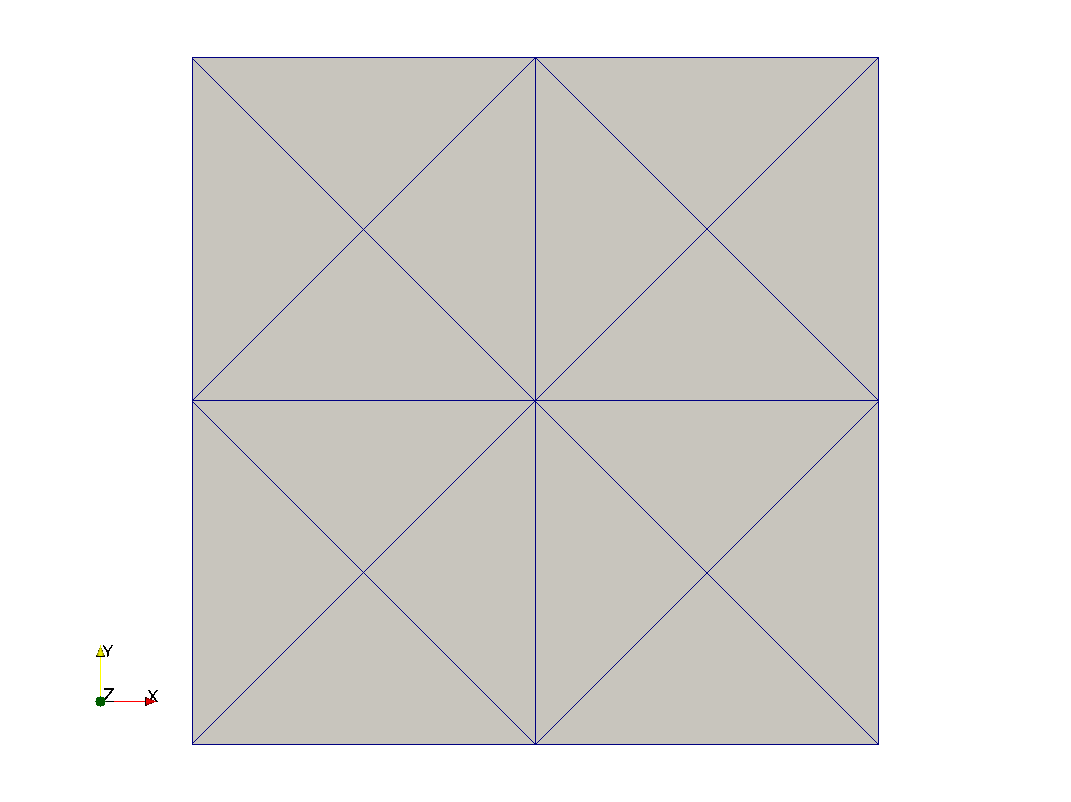
\includegraphics[width=7cm]{python_codes/fieldstone_131/example1/example1}
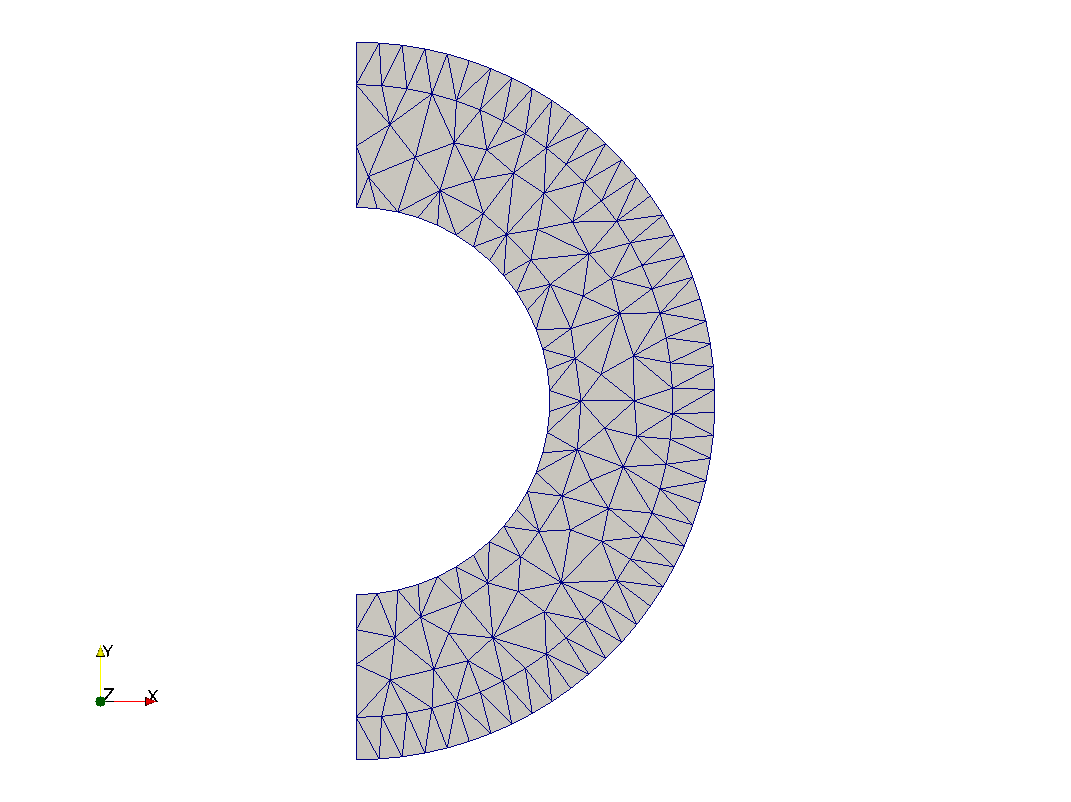
\includegraphics[width=7cm]{python_codes/fieldstone_131/example2/example2}\\
{\captionfont Example 1 (left), example 2 (right)}
\end{center}


\begin{center}
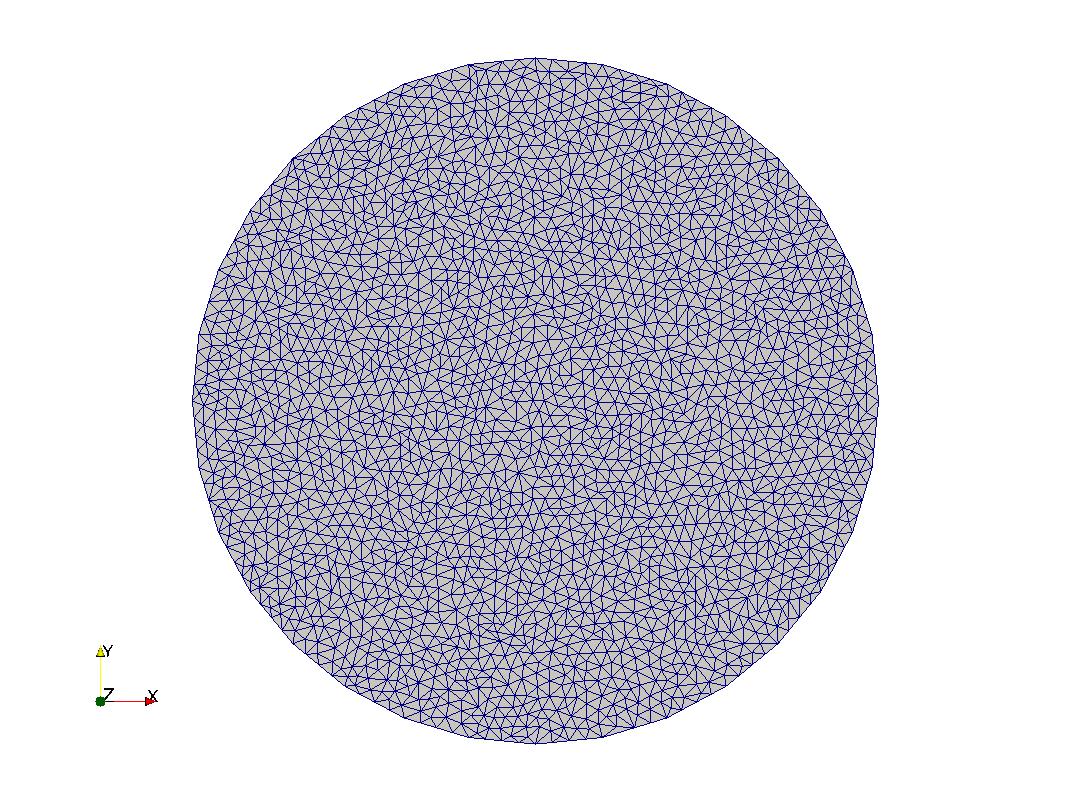
\includegraphics[width=7cm]{python_codes/fieldstone_131/example3/example3}
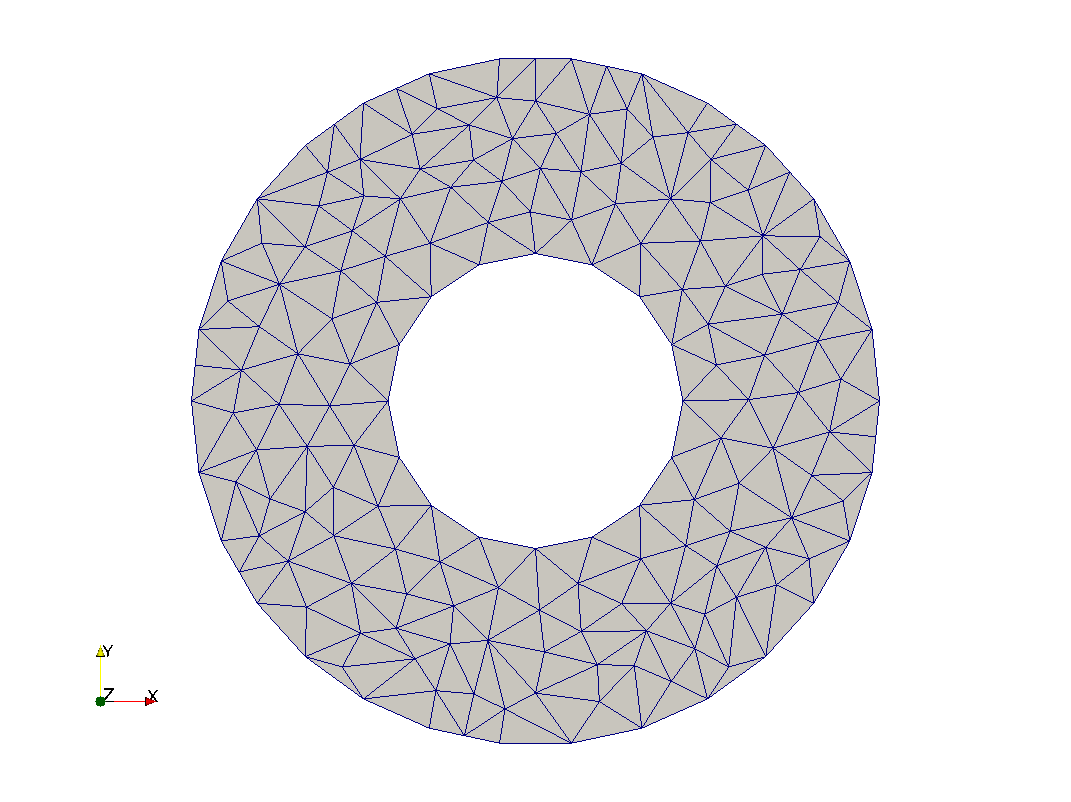
\includegraphics[width=7cm]{python_codes/fieldstone_131/example4/example4}\\
{\captionfont Example 3 (left), example 4 (right)}
\end{center}

\begin{center}
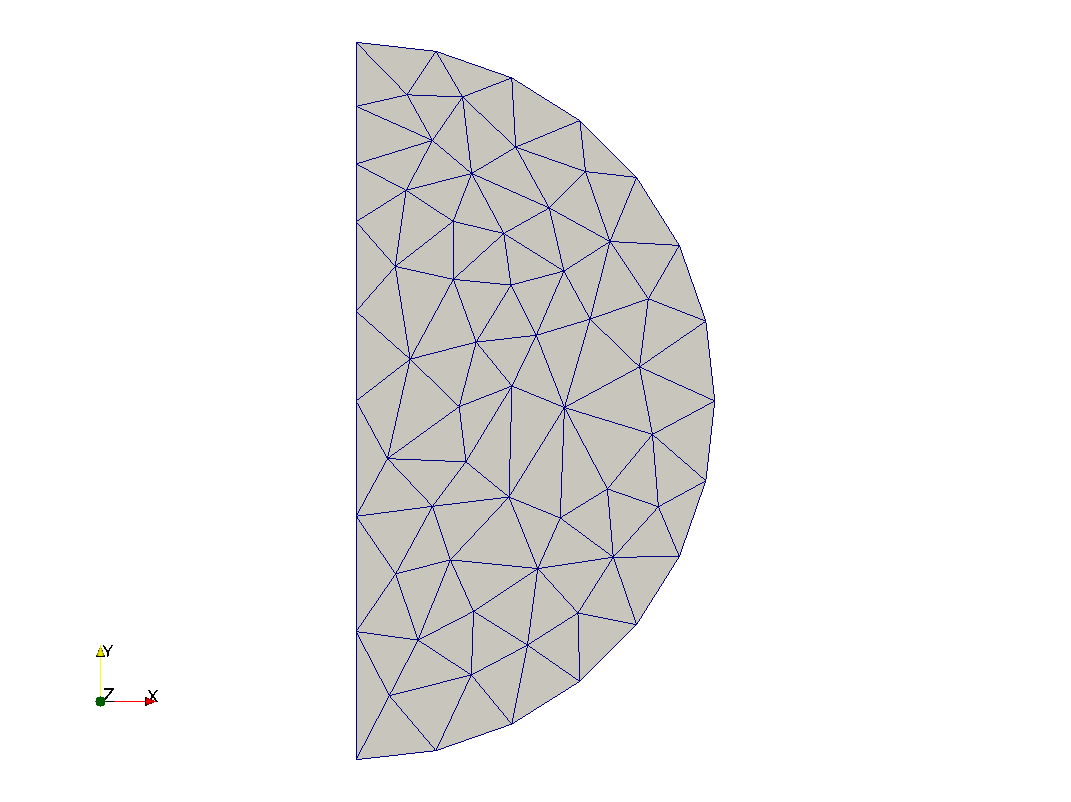
\includegraphics[width=7cm]{python_codes/fieldstone_131/example5/example5}
{\captionfont Example 5 (left), example 6 (right)}
\end{center}
